 %%\documentclass[12pt]{article}
 %\usepackage{epsfig}
%%  \textwidth 6.0in
 %% \textheight 9.2 in
 % \pagestyle{empty}
 %%\topmargin -0.25truein
%% \oddsidemargin -.6truein
%% \evensidemargin -.6truein
%% \parindent=1.5pc
%% \baselineskip=15pt

%%\newcommand{\oot}{\overline {126}}
%\documentclass[12pt]{article}	%%
%\baselineskip=7mm		%%
%\def\baselinestretch{1.2}	%%
%\usepackage[left=0.75in,top=0.6in,right=0.75in,bottom=0.6in]{geometry}


\documentclass[aps,onecolumn,showpacs,superscriptaddress,groupedaddress,nofootinbib,preprint]{revtex4-1}
\pdfoutput=1

\usepackage{slashed}
\usepackage{bm}        % for math
\usepackage{amssymb}   % for math
\usepackage{amsmath}
\usepackage{graphicx,psfrag,amsmath,subfigure}
\usepackage[colorlinks]{hyperref}
\usepackage{rotating}
\usepackage{units}
\newcommand{\beqa}{\begin{eqnarray}}
\newcommand{\eeqa}{\end{eqnarray}}

\newcommand{\be}{\begin{equation}}
\newcommand{\ee}{\end{equation}}
\newcommand{\cl}{\%\,\,  \text{C.L.}}
\begin{document}
\title{On finding collider-stable particles using Machine Learning}
 
\author{Charanjit K. Khosa, Veronica Sanz and Michael Soughton} 
%\email{V.Sanz@sussex.ac.uk}
%\email{ck373@sussex.ac.uk}
\affiliation{Department of Physics and Astronomy, University of Sussex, 
Brighton BN1 9QH, UK}
\date{\today}

\maketitle 

\section{Introduction}
Collider searches for dark matter are one of the important avenues for new physics searches at Large Hadron Collider(LHC). It 
 includes mono(visible) objects and missing transverse energy channels where this single object could be a jet, W, top quark, 
photon or $ t \bar t $ pair. This basic idea for these channels is the momentum mismatch in the final state i.e. these mentioned 
objects recoil against nothing. Like other new physics searches at LHC, these channels also face huge SM backgrounds, 
but additionally  contamination by  collider stable particles. 

Collider stable particles could manifest themselves as missing momentum, mimicking dark matter particles. To see the 
unknowns in the LHC data, it is extremely important to remove this degeneracy. This task is even more challenging than
 analyzing the signal and background for the DM searches because here we are concerned with the two or more(unknown) new 
 physics models. The decay width of the particle is a parameter of its mass which we do not know a priori. In this situation, one would like to 
 design a search template with respect to the better understood new physics model. This complex analysis certainly requires the implementation of new (more sophisticated) techniques beyond  conventional search strategies. This calls for the use of machine learning algorithms which are emerging as a suitable platform for exploring a co-relations in multi-dimensional parameter space.

Axions like particles(ALPs) is the 
typically example of collider stable particles. ALPs could be present in many theoretically well motivated models. Depending on 
the model details, different mass and coupling range is possible for these particles. ALPs themselves could be dark matter particle\cite{} or
 can be a dark matter mediator. These exotic particles are constrained by many collider searches in addition to 
 the astrophysical constraints. In fact, collider constraints are complementary to the astrophysical constraints\cite{}. The direct 
 axion search experiments are designed to target their couplings with the photons. ALPs could look like MET if they decay outside the detector volume.
 
At present, LHC dark matter searches are interpreted using simplified dark matter models

We are using Machine Learning to compare the features of dark matter(DM) signals from BSM models,
specifically Axion-Like Particles (ALPs) Effective Field Theory \cite{Mimasu:2014nea,Brivio:2017ije}, a simplified DM model with a
spin-1 mediator [2] as well as WHICH SUSY MODEL? We are comparing signal 1 versus 
signal 2 with the assumption that we understand the background very well. 

Collider stable axion like particles and other dark matter candidates.

Paper is organised as follows:

\begin{figure}
\centering
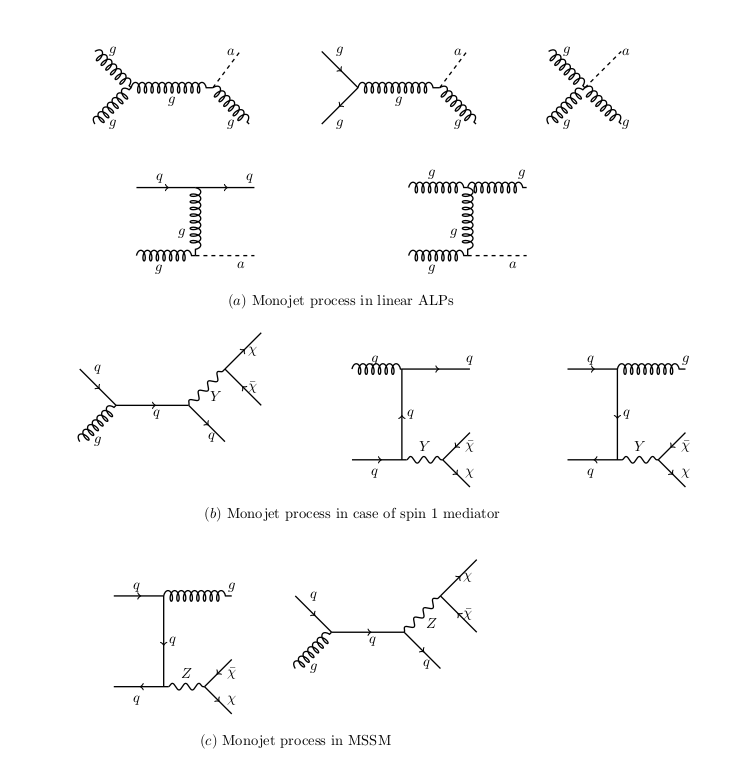
\includegraphics[scale=0.35]{draftfig/fyndiag.png}
\caption{Feynman diagrams for mono-jet process in Linear ALPs case (fermion-axion couplings are not considered), spin 1 mediator and in MSSM\label{fyndiag}.}
\end{figure}

\section{Benchmark processes}
We generate parton level events for mono jet and  dijet processes  for centre of mass energy $\sqrt{s}=14$ TeV. In case of monojet, $p_T^j > 130$ GeV and for dijet $p_T^j > 30$ GeV is demanded. We construct the following kinematical variables for these processes
\begin{itemize}
\item Monojet : $p_T^j$ (MET) ,$\eta_j$, $\phi_j$
\item Dijet : $p_T^{j_1}$, $p_T^{j_2}$, $\eta_{j_1}$, $\eta_{j_2}$, MET, $\Delta \phi_{jj}$, $\Delta \phi_{MET j_1}$, $\Delta \phi_{MET j_2}$
\end{itemize}
here $j_1$ and $j_2$ refer to the leading and sub-leading jet respectivly. For the signal we consider three cases; (1) when dark matter candidate is collider stable particle (2) when dark matter is produced from the decay of the heavy mediator, (3) weakly interacting massive particle in the R-parity conserving supersymmetric scenario. Feynman diagrams for mono-jet process in these cases are shown in Figure \ref{fyndiag}. 

\subsection{Axion like particles}

\begin{align}\label{eqn:L_eff}
    \mathcal{L}_a = &\frac{1}{2}\partial_{\mu}a\,\partial^{\mu}a  - \frac{1}{2}M_{a}^2 a^2
                  -\frac{g_{a\gamma}}{4}a\,F_{\mu\nu}\tilde{F}^{\mu\nu} \nonumber 
                   - \frac{g_{agg}}{2}a\,\text{Tr}\left[G_{\mu\nu}\tilde{G}^{\mu\nu}\right] 
                  +\sum_{\psi}g^{\psi}_{a} \,m_\psi\,a\bar \psi \gamma^5 \psi\,,
                   % +\,ig_{ah}\left(\Phi^{\dagger}\overleftrightarrow{D}_{\mu}\Phi\right)\partial^{\mu}a\,,
\end{align}
ALP-gluon coupling \cite{Mimasu:2014nea,Brivio:2017ije} :
\[
g_{agg} \lesssim \unit[1.1\cdot10^{-5}]{GeV^{-1}} \quad (90\cl) \quad \text{for}\quad m_a \lesssim \unit[60]{MeV}\,.
\]

\[ f_a=1\,\, \mbox{TeV} \quad \quad  M_{a}=1\,\, \mbox{MeV}  \]

We used linear axion like particle(ALP) feynrule model available in the literature\cite{linearalps}. 

\begin{figure}
\centering
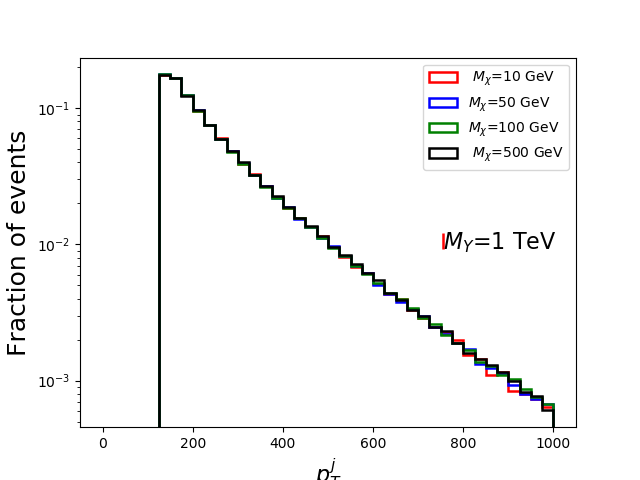
\includegraphics[scale=0.40]{draftfig/ptjS1med1tev.png}
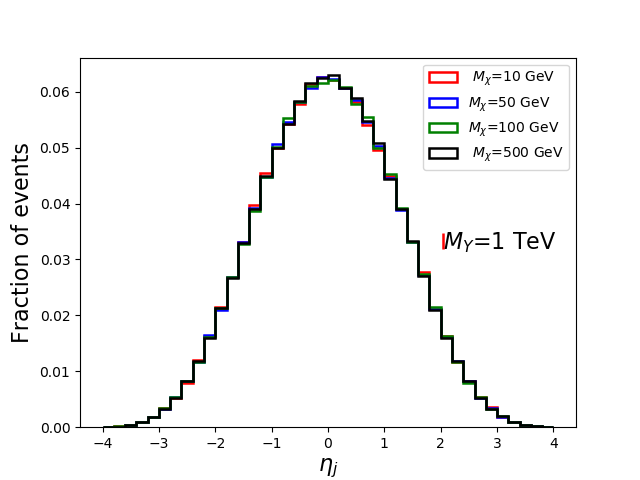
\includegraphics[scale=0.40]{draftfig/etajS1med1tev.png}
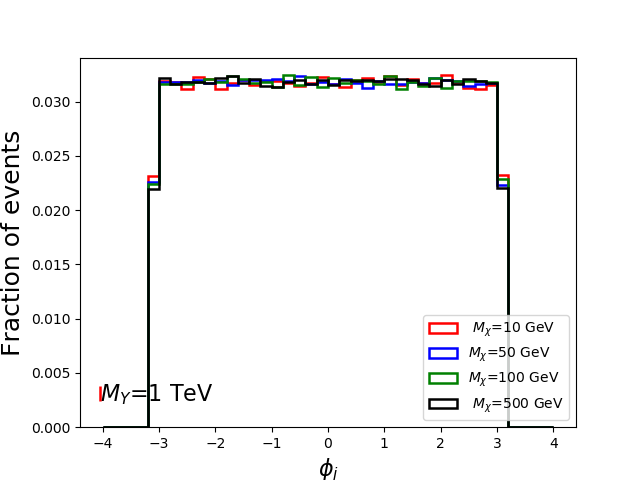
\includegraphics[scale=0.40]{draftfig/phijS1med1tev.png}
\caption{$p_T$, $\eta$, $\phi$ distributions for the monojet  in case of  spin-1 mediator (at parton level)\label{spin1med}.}
\end{figure}




\subsection{Simplified Models : Spin 1 Mediator}
We used DMSimp\cite{} model to generate the events. We focus on the heavy mediator case. Once the mediator is heavy enough to produce the 
dark matter then kinematics is not very sensitive to the dark matter mass as shown in Fig. \ref{spin1med}. For further analysis, we use 
 $M_Y=1\,\, \mbox{TeV}$ and  $M_{\chi}=10\,\, \mbox{GeV}$ mass parametes.

\subsection{WIMP : Susy}



\begin{figure}
\centering
\includegraphics[scale=0.40]{draftfig/ptjallsignal.png}
\includegraphics[scale=0.40]{draftfig/etajallsignal.png}
\includegraphics[scale=0.40]{draftfig/phijallsignal.png}
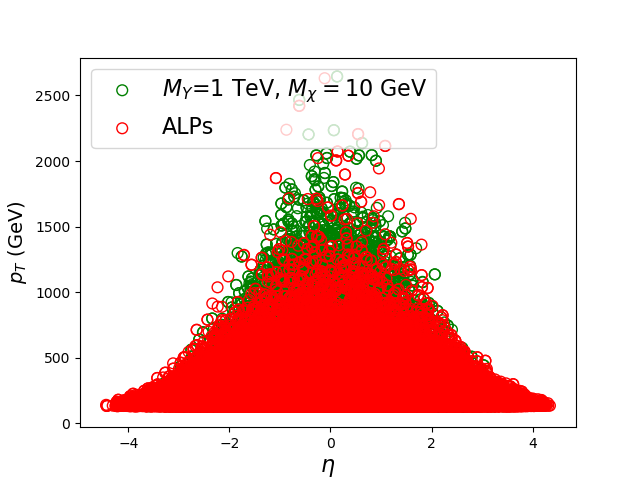
\includegraphics[scale=0.40]{draftfig/ptjetajaxspin1.png}
\caption{1D and 2D histograms for the monojet process for linear ALPs versus spin-1 mediator case (at parton level).}
\end{figure}






\begin{figure}
\centering
\includegraphics[scale=0.30]{draftfig/axion/dijet/ptj1axspin1.png}
\includegraphics[scale=0.30]{draftfig/axion/dijet/ptj2axspin1.png}
\includegraphics[scale=0.30]{draftfig/axion/dijet/etaj1axspin1.png}
\includegraphics[scale=0.30]{draftfig/axion/dijet/etaj2axspin1.png}
\includegraphics[scale=0.30]{draftfig/axion/dijet/metaxspin1.png}
\includegraphics[scale=0.30]{draftfig/axion/dijet/deltaphijjaxspin1.png}
\includegraphics[scale=0.30]{draftfig/axion/dijet/dphimetj1axspin1.png}
\includegraphics[scale=0.30]{draftfig/axion/dijet/dphimetj2axspin1.png}
\caption{Linear ALPs, di-jet}
\end{figure}





\begin{figure}
\centering
\includegraphics[scale=0.40]{draftfig/ROCsignalLRandNN.png}
%\includegraphics[scale=0.40]{draftfig/ROCDNN.pdf}
\caption{ROC curves using logistic regression and neural network (with 10 hidden layer) for ALPs versus EFT and ALPs versus WIMPs.}
\end{figure}

\section{Supervised Classification}

\subsection{Logistic regression} 
SGDclassifier : $\lambda= 10^{-5}$
\subsection{NN-kinematic features}
Next, We investigate the classification accuracy using  neural networks with the same input 
features i.e. $p_T$ and $\eta$ of the jet. We used 5 (fully connected) hidden layers for the  network as including more layers does not improve the performance. or the intermediate layers, ReLU activation function is used and we considered binary cross entropy loss function.
\subsection{NN-2D histograms}
We construct 2D histograms using $p_T$ and $\eta_j$ of the jet, using N number of events. A few illustrative pictures of these plots are 
shown in figure \ref{demopic}. We consider $p_T$ and $\eta$ in range [100, 2000] GeV and -4to 4 respectively with a 29 $\times$ 29 grid. We use the information of density in this grid as an input of 
NN (2 fully connected hidden layers). In figure \ref{accuracy1}, we show the performance dependence on the number of events injected in one picture. This plot is 
based on the fixed data sample. More explicitly, the number of data points NN is trained and tested is less in the case where we have more events per image.

For a data sample, when we consider images with 50 events per image, we checked the performance of NN by varying the number of bins in the grid. We get 
the same accuracy until 5 $\times$ 5 bins in the grid although there is a huge reduction in the number of parameters involved in the algorithm.
\subsection{CNN}
We also used convolution neural network for the 2D histograms, with 2 convolution layers, 2 max-pooling layers and one dense 
flatten hidden layers, ReLu activation function for all the cases.

\begin{figure}
\centering
\includegraphics[scale=0.40]{draftfig/proc1i1.png}
\includegraphics[scale=0.40]{draftfig/proc1i2.png}
\includegraphics[scale=0.40]{draftfig/proc2i1.png}
\includegraphics[scale=0.40]{draftfig/proc2i2.png}
\caption{Illustrative 2D histograms for the two processes averaging over 100K events. Upper and lower row represents process 1 and 2 respectively. mention the processes not 1 and 2.}\label{demopic}
\end{figure}




\section{Unsupervised learning}

\section{Need to understand}
What is the correct approach to use multi-dimensional probability information ?

What about the density estimates which experimentalists were discussing at ICTP workshop.

\section{steps}
\begin{itemize}
\item Compare the single image ROC with NN, CNN, etc
\item plot of accuracy versus number of bins
\item LO vs NLO (QCD: ISR, FSR, loops 
\item May be important backgrounds
\end{itemize}

\begin{figure}
\centering
\includegraphics[scale=0.60]{draftfig/acVsNevents.pdf}
\caption{Accuracy versus images with varying number of events (fully connected NN with 2 hidden layers) in a 29 $\times$ 29 grid.}\label{accuracy1}
\end{figure}

In figure \ref{accuracy1}, we are providing the information of approximate or exact likelihood function to NN (depending on how many events per image are considered). 

\section{Conclusions}

In this paper, we ...

\section{Meeting on 1st May}
1.Try the same plot with more event data (say 800K), 2. fix the data sample, i.e. number of images and vary the no of events per image and check the performance.
3. Try same plot with CNN. 4. check the accuracy for 1 event may be with 50K images...following this approach we might understand bias-variance trade off in context 
of collider data...We need to combine all the ROC curve for various approaches...for this project we will also provide number of parameters information.

\section{Meeting on 3rd May}
We will do detector simulation for the same benchmarks and also for the heavy dark matter masses in case of WIMP.


\section{Steps from 28/06 onwards}
\begin{itemize}
	\item Investigate the DM mass dependence further (would be nice to have a ROC curve with different masses but this seems pointless if there is no difference)
	\item Create larger samples to check if a VAE will work (should be running on Oracle soon)
	\item Investigate NLO processes and see if model accuracy is increased. We could find $\sigma_\mathrm{LO}^\mathrm{1j}/\sigma_\mathrm{NLO}^\mathrm{2j}$ (why is this useful?) and also use backgrounds (mostly p p $>$ Z j with p p $>$ W j) - given in \cite{Barducci:2015ffa}. Although it would be great to use a real background, I don't think it absolutely necessary to show the usefulness of the ML algorithms we are using.
	\item Make the plot of accuracy vs Nevents/image for various fixed Nimages
\end{itemize}

Should this then be enough to write up?


\section{acknowledgments}
%\begin{acknowledgments}
C.K.K. wishes to acknowledge support from the Royal Society-SERB Newton International Fellowship (NF171488). 
The work of V.S. by the Science Technology and Facilities Council (STFC) under grant number
ST/P000819/1.
%\end{acknowledgments}


\begin{thebibliography}{99}
\bibitem{linearalps} 
http://feynrules.irmp.ucl.ac.be/wiki/ALPsEFT

\bibitem{Mimasu:2014nea}
  K.~Mimasu and V.~Sanz,
  %``ALPs at Colliders,''
  JHEP {\bf 1506} (2015) 173,
%  doi:10.1007/JHEP06(2015)173
  [arXiv:1409.4792 [hep-ph]].
  %%CITATION = doi:10.1007/JHEP06(2015)173;%%



\bibitem{Brivio:2017ije}
  I.~Brivio, M.~B.~Gavela, L.~Merlo, K.~Mimasu, J.~M.~No, R.~del Rey and V.~Sanz,
  %``ALPs Effective Field Theory and Collider Signatures,''
  Eur.\ Phys.\ J.\ C {\bf 77} (2017) no.8,  572,
%  doi:10.1140/epjc/s10052-017-5111-3
  [arXiv:1701.05379 [hep-ph]].
  %%CITATION = doi:10.1140/epjc/s10052-017-5111-3;%%
  %37 citations counted in INSPIRE as of 08 Mar 2019


%\cite{Freitas:2019hbk}
\bibitem{Freitas:2019hbk}
  F.~F.~Freitas, C.~K.~Khosa and V.~Sanz,
  %``Exploring SMEFT in VH with Machine Learning,''
  arXiv:1902.05803 [hep-ph].
  %%CITATION = ARXIV:1902.05803;%%

\end{thebibliography}

\end{document}




